\section{Conceptos fundamentales de la teor\'ia cin\'etica y transporte en el Plasma}

\subsection{Derivaci\'on Heur\'istica de la Ecuaci\'on Cin\'etica}

Para la derivaci\'on de la ecuaci\'on cin\'eca o la ecuaci\'on de Boltzmann seguimos la siguiente estrategia tal y como lo plantea \cite{freidberg2014}

\begin{enumerate}
  \item Derivar la conservaci\'on de part\'iculas de un fluido simple. En un espacio de fase 3-D.
  \item Generalizar a 6-D y divir las interacciones en aquellas de corto y largo alcance.
  \item A\~nadir el efecto de colisiones donde se asume \'unicamente \textbf{colisiones binarias}.
\end{enumerate} 

\subsubsection{Conservaci\'on de part\'iculas en un espacio de fase 3-D}

Primero consideraremos el caso 1-D sin fuentes ni sumideros en tal caso para un elemento infinitesimal de volumen 

\begin{equation*}
\text{Part\'iculas ganadas} = \text{Part\'iculas que entran - Part\'iculas que salen}
\end{equation*}

Sea $n(x_1, t)$ la densidad de part\'iculas y $\Gamma_{x_1} = nv_{x_1}$ el flujo de part\'iculas que entran al volumen.  

\begin{eqnarray}
  \text{Part\'iculas ganadas en un tiempo }  \Delta t &=& [n(x_1, t + \Delta t) - n(x_1,t)]\Delta x_1\Delta x_2\Delta x_3 \nonumber \\
  \text{Part\'iculas entran en un tiempo } \Delta t &=& (\text{flujo que entra})(\text{\'area})\Delta t = \Gamma_{x_1}\big{|}_{x_1 - \Delta x_1/2} \Delta x_2\Delta x_3 \nonumber\\
  \text{Part\'iculas salen en un tiempo } \Delta t &=& (\text{flujo que sale})(\text{\'area})\Delta t = \Gamma_{x_1}\big{|}_{x_1 + \Delta x_1/2}\Delta x_2\Delta x_3 \nonumber\\
\end{eqnarray}

\begin{figure}[htb!]
  \centering
  \label{fig:box}
  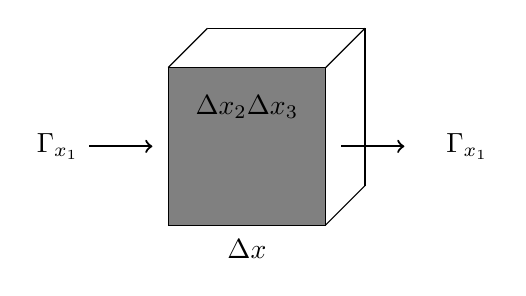
\begin{tikzpicture}
    \node at (-1.4,1) {$\Gamma_{x_1}$};
    \draw[->, thick] (-1,1) -- (-0.2,1);
    \draw[->, thick] (2.2, 1) -- (3,1);
    \node at (3.8,1) {$\Gamma_{x_1}$};
    \fill[gray] (0,0) rectangle (2,2);
    \draw (0,0) rectangle (2,2);
    \draw (2, 0) -- (2.5,0.5);
    \draw (2.5,0.5) -- (2.5, 2.5);
    \draw (0.5,2.5) -- (2.5,2.5);
    \draw (0,2) -- (0.5,2.5);
    \draw (2,2) -- (2.5,2.5);
    \node at (1,-0.3) {$\Delta x$};
    \node at (1, 1.5) {$\Delta x_2 \Delta x_3$};
  \end{tikzpicture}
  \caption{Elemento de volumen en un espacio de fase 3-D con un flujo en la direcci\'on $x_1$.}
\end{figure}

Expandiendo las expresiones en series de Taylor a primer orden

\begin{eqnarray}
  \text{Ganadas }\Delta t &=& [ n(x_1,t) + \partial_t n(x_1,t) - n(x_1, t)]\Delta x_1\Delta x_2\Delta x_3 \nonumber\\ 
                          &=& \left\{ \left[\Gamma_{x_1}\big{|}_{x_1} - \frac{\Delta x}{2}\partial_{x_1}(\Gamma_{x_1})\big{|}_{x_1}] - [\Gamma_{x_1}\big{|}_{x_1} + \frac{\Delta x}{2}\partial_{x_1}(\Gamma_{x_1})\big{|}_{x_1}\right]\right\}\Delta x_2\Delta x_3\nonumber
  \end{eqnarray}

De all\'i se obtiene la expresi\'on

\begin{equation*}
  \partial_{t} n = -\partial_{x_1}\Gamma_{x_1}
\end{equation*}

La generalizaci\'on al caso 3-D es inmediata, tal que 

\begin{equation*}
  \partial_t n(\textbf{x}, t) + \nabla_\textbf{x}\cdot\pmb{\Gamma}(\textbf{x},t) = 0
\end{equation*}

\subsubsection{Generalizaci\'on a un espacio de fase 6-D}

En un espacio de fase 6-D conformado por los puntos (\textbf{x}, \textbf{v}) se procede a generalizar de forma que 

\begin{eqnarray*}
  n(\textbf{x},t) \rightarrow f(\textbf{x}, \textbf{v},t) \text{ (6-D) } \quad \quad \quad \quad \text{densidad del espacio de fase}\\
  \Delta x_1\Delta x_2\Delta x_3 \rightarrow \Delta x_{1}\Delta x_2\Delta x_3\Delta v_{x_1}\Delta v_{x_2}\Delta v_{x_3} \text{ (6-D) } \text{elemento de volumen}
\end{eqnarray*}

N\'otese la independencia entre $\textbf{x}$ y $\textbf{v}$, por lo que en general $\textbf{a} = \textbf{a}(\textbf{x},\textbf{v}, t)$. Ahora generalizamos tomando en cuenta fuentes y sumideros para cada elemento del volumen del espacio de fase. Primero se considerara el caso donde solo haya moviento en el espacio de fase en las direcciones $x_1$ y $v_{1}$, luego, de manera an\'aloga al caso en el espacio 3-D ser\'a f\'acil generalizar las expresiones. Imaginemos al espacio f\'isico y al espacio de velocidades la geometr\'ia del problema est\'a dada por 

\begin{figure}[h!]
  \label{fig:fasespace}
  \centering
  \begin{subfigure}{0.49\textwidth}
    \begin{tikzpicture}
      \draw (0,0) rectangle (3,2);
      \node at (-1.4,1) {$v_{1}$};
      \draw[->, thick] (-1, 1) -- (-0, 1);
      \draw[->, thick] (3,1) -- (4,1);
      \node at (4.4,1) {$v_{1}$};
      \node at (0,-0.5) {$x_1 - \Delta x_1/2 $};
      \node at (3,-0.5) {$x_1 + \Delta x_1/2 $};
    \end{tikzpicture}
    \caption{}
  \end{subfigure}
  \begin{subfigure}{0.49\textwidth}
    \begin{tikzpicture}
      \draw (0,0) rectangle (3,2);
      \node at (-1.4,1) {$a_{1}$};
      \draw[->, thick] (-1, 1) -- (-0, 1);
      \draw[->, thick] (3,1) -- (4,1);
      \node at (4.4,1) {$a_{1}$};
      \node at (0,-0.5) {$v_{1} - \Delta v_{1}/2 $};
      \node at (3,-0.5) {$v_{1} + \Delta v_{1}/2 $};
    \end{tikzpicture}
    \caption{}
  \end{subfigure}
  \caption{(a) flujo de part\'icula en el espacio f\'isico. (b) flujo de part\'iculas en el espacio de velocidades.}
\end{figure}

\begin{equation*}
  \text{part\'iculas ganadas} = \text{entran} - \text{salen} + \text{fuentes} - \text{sumideros}
\end{equation*}

De está definimos

\begin{eqnarray}
  \text{ganadas en } \Delta t &=& [f(x_1, v_{1}, t + \Delta t) - f(x_1, v_{1}, t)]\Delta\textbf{r}\Delta\textbf{v}\nonumber\\
  \text{entran en espacio f\'isico} &=& \Delta x_{2}\Delta x_{3}\Delta t[v_{1}fd\textbf{v}]_{x_1 - \Delta x_1/2} \nonumber\\
  \text{salen en espacio f\'isico} &=& \Delta x_{2}\Delta x_{3}\Delta t[v_{1}fd\textbf{v}]_{x_1 + \Delta x_1/2} \nonumber\\
  \text{aceleran en espacio de velocidad} &=& \Delta v_{2}\Delta v_{3}\Delta t[a_{x_1}fd\textbf{r}]_{v_{1} - \Delta v_{1}/2} \nonumber\\
  \text{aceleran fuera del espacio de velocidad} &=& \Delta v_{2}\Delta v_{3}\Delta t[a_{x_1}fd\textbf{x}]_{v_{1} + \Delta v_{1}/2} \nonumber\\
  \text{fuentes} - \text{sumideros} &=& s\Delta \textbf{x} \Delta\textbf{v}\Delta t \nonumber
\end{eqnarray}

Al aplicar las correspondientes expansiones de Taylor al rededor de $t$, $x_1$ y $v_1$ se obtiene 

\begin{equation*}
  \partial_t f = -\partial_{1}(v_1 f) - \partial_{v_1} (a_1 f) + s
\end{equation*}

Adem\'as recordando que $\partial_{1}v_i = s$ se obtiene

\begin{equation*}
  \partial_t f + v_1\partial_{1}f + a_1\partial_{v_1} f + f\partial_{v_1}a_1 = s
\end{equation*}
  
La generalizaci\'on al espacio 6-D es simple tal que 

\begin{equation*}
  \partial_t f(\textbf{x},\textbf{v}, t) + \textbf{v}\cdot\nabla f(\textbf{x}, \textbf{v}, t) + \textbf{a}\cdot\nabla_{\textbf{v}} f(\textbf{x}, \textbf{v}, t)= -f(\textbf{x}, \textbf{v}, t)\nabla_\textbf{v}\cdot \textbf{a} + s 
\end{equation*}

\subsubsection{Ecuaci\'on Cin\'etica de Boltzmann}

Considerando el caso de inter\'es, el plasma, el t\'ermino $\textbf{a}$ puede ser dividido en dos partes, aceleraci\'on por interacciones de corto alcance $\textbf{a}_c$ y por interacciones de largo alcance $\textbf{a}_l$ tal que 

\begin{equation*}
  \textbf{a} = \textbf{a}_s + \textbf{a}_l
\end{equation*}

El cr\'iterio para definir el alcance de las interacciones es el radio de Debye $\lambda_D$. Se c\'ataloga como una fuerza de corto alcance a aquellas que se dan en un radio mucho menor al de Debye $r \ll \lambda_D$ y en este caso se asumen solo colisiones de Coulomb las cuales debido al apantallamiento de Debye son despreciales fuera de la esfera de Debye $V_D$. 

La segunda aproximaci\'on que se introduce es que se limitan las colisiones a ocurrir en un punto tan pequeño que la posici\'on de la part\'icula no cambia en el espacio f\'isico ni antes ni despu\'es de una colisi\'on. Adem\'as, la velocidad de la part\'icula cambia finitamente. Es decir, el resultado de una colisi\'on no puede hacer que la velocidad se dispare al infinito. Entonces consideramos, una colisi\'on en un espacio de fase 6-D implica que $\textbf{x}$ no cambia y $\textbf{v}$ puede salir del elemento de volumen en el espacio de velocidades, es decir, el momento de la part\'icula cambia. 

Por otro lado, se desprecian los efectos de las colisiones. Tambi\'en se asume que el n\'umero de part\'iculas en un $V_D$ este dentro del l\'imite estad\'istico. Y las escalas dimensionales y temporales del problema son tales que $V_D \ll L$ y $\tau \ll \tau_{pe}$ donde $\tau_{pe}$ es el periodo electr\'onico del plasma. 

Consideremos primero las interacciones de largo alcance

\begin{equation*}
  \textbf{a}_{l,\alpha} = \frac{Ze}{m_\alpha}(\textbf{E} + \textbf{v}\times\textbf{B})
\end{equation*}

Para estas interacciones de largo alcance se toma solo el promedio tal que los campos sean suaves y no var\'ien abruptamente, por lo que $\textbf{E}$ y $\textbf{B}$ solo dependen de $\textbf{x}$. De all\'i que

\begin{eqnarray}
  \nabla_\textbf{v}\cdot\textbf{a}_{l, \alpha} &=& \frac{Ze}{m_\alpha}\nabla_\textbf{v}\cdot(\textbf{E}(\textbf{x},t) + \textbf{v}\times\textbf{B}(\textbf{x},t))\nonumber\\
                                   &=& \frac{Ze}{m_\alpha}\left[\nabla_\textbf{v}\cdot \textbf{E} + \nabla_\textbf{v}\cdot(\textbf{v}\times\textbf{B})\right] \nonumber\\
                                   &=& \frac{Ze}{m_\alpha}[\partial_{v_\mu} (\epsilon_{\mu\nu\rho} v_{\nu}B_{\rho})] \nonumber \\
                                   &=& \frac{Ze}{m_\alpha}\epsilon_{\mu\nu\rho}(B_\rho \partial_{v_\mu}v_{\nu} + v_\nu\cancel{\partial_{v_\mu}B_\rho}) \nonumber \\
                                   &=& \frac{Ze}{m_\alpha}\epsilon_{\mu\nu\rho}(B_\rho\delta_{\mu\nu})\nonumber \\
                                   &=& \frac{Ze}{m_\alpha}\cancel{\epsilon_{\mu\mu\rho}}B_\rho = 0
\end{eqnarray}

Bajo los supuestos anteriores, y agregando las interacciones de corto alcance como las \'unicas fuentes y/o sumideros para part\'iculas de la especie $\alpha$, la funci\'on de distribuci\'on cumple 

\begin{equation}
  \partial_t f_\alpha + \textbf{v}\cdot\nabla f_\alpha + \frac{Ze}{m_\alpha}(\textbf{E} + \textbf{v}\times\textbf{B})\cdot\nabla f_\alpha = C_\alpha
\end{equation}

Aqu\'i se reemplazo el t\'ermino de fuentes y sumideros por $s = C_\alpha$ que toma en cuenta \'unicamente colisiones binarias tal que, siendo $C_\alpha$ el operador de colisiones

\begin{equation}
  s \equiv C_\alpha = (\delta_t f_\alpha)_c = \sum_\alpha C_{\alpha\beta}(\textbf{x}, \textbf{v},t)
\end{equation}

donde $C_{\alpha\beta}$ representa el cambio en $f_\alpha$ debido a colisiones con las especies $\beta$. Es importante notar que todas las interacciones entre part\'iculas a nivel microsc\'opico se toman en cuenta dentro del operador de colisiones.


\subsection{Teor\'ia Cin\'etica y Transporte}

Los gases ionizados pueden ser espec\'ificados por una funci\'on de distribuci\'on $f_\alpha$(\textbf{x}, \textbf{v}, t). Como vimos en el apartado anterior

  \begin{equation}\label{eq:k}
    \frac{df_\alpha}{dt} \equiv \left(\partial_t + \textbf{v}\cdot\nabla + \frac{Z_\alpha e}{m_\alpha}(\textbf{E} + \textbf{v}\times\textbf{B})\cdot \nabla_\textbf{v} \right)f_\alpha = C_\alpha
  \end{equation}

  \textbf{Esta ecuaci\'on no toma en cuenta fluctuaciones termicas}; es decir, a pesar de no conocer cada part\'icula del sistema por lo que se debe modelar como un conjunto de variables aleatorias, asumimos un n\'umero de part\'iculas lo suficientemente grande para que la varianza entre las cantidades macrosc\'opicas sea negligible y tengamos propiedades f\'isicas bien definidas como Temperatura y presi\'on. La funci\'on de distribuci\'on representa densidades suaves promediadas sobre un elemento de volumen. Los campos $\textbf{E}$ y $\textbf{B}$ tambi\'en varian suavemente, no hay fluctuaciones r\'apidas de microcampos y microfuerzas, es decir, se toma el promedio de esos campos cuyas interacciones son de largo alcance. Los efectos de interacciones a corto alcance se consideran solo en el t\'ermino de colisiones $C_\alpha$ asumiendo \'unicamente colisiones binarias.

  Ahora de la mec\'anica est\'istica es posible obtener los momentos de una distribuci\'on, nos interesa el primer y segundo momento\cite{helander2005} de la distribuci\'on definidos como 

  \begin{equation}
    n_\alpha\left<g_k\right> \equiv \int d^3 g_k f
  \end{equation}

  Donde $g_k$ est\'a dado por $\text{const} \cdot m_\alpha\textbf{v}^k$. De ah\'i obtenemos las siguentes expresiones 

  \begin{eqnarray}
    n_\alpha &=& \int d^3v f_\alpha \label{eq:dens}\\
    \textbf{u}_{\alpha} &=& \frac{1}{n_\alpha}\int d^3v f_\alpha\textbf{v} \label{eq:vel} \\
    \textbf{Q}_\alpha &\equiv& \frac{m_\alpha n_\alpha \left<v^2\textbf{v}\right>}{2}\label{eq:heat}
  \end{eqnarray}

El momento cero en la Ec. \eqref{eq:dens} es la densidad de part\'iculas de una especie en el plasma, i.e., el n\'umero de part\'iculas de una especie por unidad de volumen. El primer momento Ec.\eqref{eq:vel} es la velocidad promedio de las part\'iculas de una especie en el plasma. La Ec.\eqref{eq:heat} es el flujo de energ\'ia. 

  Ahora definimos el flujo de part\'iculas en el plasma como 
  
  \begin{equation}
    \pmb{\Gamma}_\alpha \equiv n_\alpha\textbf{u}_\alpha
  \end{equation}

  De la ecuaci\'on cin\'etica es posible obtener informaci\'on y expresiones \'utiles en el contexto del plasma tal que\cite{freidberg2014}

  \begin{equation}\label{eq:moments}
    \int d^3v g_k\left[\frac{df_\alpha}{dt} - C_\alpha\right] = 0
  \end{equation}

  
\textbf{Momento 0:}
		
Para el momento cero, usando \eqref{eq:moments} con $g_k = g_0 = 1$
		
	  \begin{eqnarray*}
      \int d^3v\frac{\partial f_\alpha}{\partial t} + \int \textbf{v}\cdot \nabla f_\alpha d^3v + \int d^3v \textbf{a}_{l,\alpha} \cdot\nabla_v f_\alpha = \int d^3v C_\alpha
		\end{eqnarray*}
		
		Tomando t\'ermino a t\'ermino la ecuaci\'on anterior, el primer t\'ermino 
		
		\begin{eqnarray*}
				\int d^3v \frac{\partial f_\alpha}{\partial t} = \frac{\partial}{\partial t}\int d^3v f_\alpha =  \frac{\partial n_\alpha}{\partial t}
		\end{eqnarray*}
		
		Para el segundo t\'ermino primero, considerando que $\nabla\cdot\textbf{v} = 0$
	
		\begin{eqnarray*}
			\nabla\cdot(\textbf{v}f_\alpha) = \textbf{v}\cdot\nabla f_\alpha + f_\alpha \cancel{\nabla\cdot\textbf{v}}^{0} \\
			\implies \textbf{v}\cdot\nabla f_\alpha = \nabla\cdot(\textbf{v}f_\alpha)
		\end{eqnarray*}
		
		Reemplazando esto en la segunda integral
		
		\begin{eqnarray*}
      \int d^3v \nabla\cdot(\textbf{v}f_\alpha) = \nabla\cdot \int d^3v \textbf{v}f_\alpha = \nabla\cdot(n_\alpha \textbf{u}_\alpha) = \nabla\cdot\pmb{\Gamma}_\alpha 
    \end{eqnarray*}
		
    Luego, para el tercer t\'ermino, como $\textbf{E}$ y $\textbf{B}$ no son dependientes de $\textbf{v}$, y como se demostr\'o considerando $\nabla_\textbf{v}\textbf{a}_{l,\alpha} = 0$

    \begin{equation*}
      \textbf{a}_{l, \alpha}\cdot \nabla_\textbf{v} f_\alpha = \nabla_\textbf{v}(\textbf{a}_{l,\alpha}f_\alpha)
    \end{equation*}
		
		Reemplazando esto en la tercera integral, se obtiene
		
		\begin{eqnarray*}
      \int_V d^3v \nabla_v\cdot(\textbf{a}_lf_\alpha) = \int_{\partial V} (\textbf{a}_{l,\alpha}f_\alpha) \cdot d\textbf{S}_v = 0
		\end{eqnarray*}	
		
    En el resultado anterior se us\'o el teorema de la divergencia de Gauss, ahora para visualizar por que se anula, recordemos que integramos sobre todo el espacio de velocidades, una de nuestras suposiciones iniciales fue que la funci\'on de distribuci\'on $f_\alpha$ deca\'ia lo suficientemente r\'apido para que en el \textbf{l\'imite infinito la probabilidad de tener velocidades infinitas tendiera a cero}, si nos imaginamos el espacio de velocidades como una esfera de radio infinito, la frontera de dicho volumen $\partial V$ debe ser tal que las velocidades en la superficie tiendan a infinito, lo que implica que $f_\alpha \rightarrow 0$, y por tanto la integral de superficie tambi\'en tender\'a a cero.

Reemplazando estos resultados en la expresi\'on \eqref{eq:moments} se obtiene la siguiente relaci\'on

  \begin{equation}\label{eq:cont}
    \partial_t n_\alpha + \nabla\cdot\pmb{\Gamma}_\alpha = S_\alpha
  \end{equation}

  donde $S_\alpha$ son las fuentes y/o sumideros de las part\'iculas $\alpha$. Tal que 
  \begin{equation}
    S_\alpha \equiv \int d^3v C_\alpha
  \end{equation}
  
  En estado estacionario como sugiere \cite{lechte2002} la Eq. \eqref{eq:cont} se reduce a 

  \begin{eqnarray*}
    \nabla\cdot\pmb{\Gamma}_\alpha = S_\alpha \\
    \implies \int_V d^3r\nabla\cdot\pmb{\Gamma}_\alpha = \int_V d^3r S_\alpha\\
    \implies \oint_{\partial V} \pmb{\Gamma}_\alpha\cdot d\textbf{S} = \int_V d^3r S_\alpha
  \end{eqnarray*}

  Definimos el flujo radial de part\'iculas como

  \begin{equation}\label{eq:rtpf}
    \Gamma_n^\alpha \equiv \oint_{\partial V} \pmb{\Gamma}_\alpha \cdot d\textbf{S} = \int_V d^3r S \approx \left<S\right>V
  \end{equation}

  Como es visible al adentrarse en balances globales, el concepto de promedios superficiales es fundamental. Conocer todos los parametros del plasma en su superficie ser\'a la piedra angular de los modelos que estamos por desarrollar.

  \begin{shaded}
    \textbf{Promedio Superficial}

    Definimos el promedio de una cantidad vectorial en la superficie como 

    \begin{equation}
      \left<\pmb{\varDelta}\right>_{\partial V} \equiv \frac{1}{A}\oint_{\partial V}\pmb{\varDelta}\cdot d\textbf{S}
    \end{equation}

    donde $A$ es el \'area superficial del plasma.
  \end{shaded}

  de lo anterior, podemos ver que el flujo radial de part\'iculas es simplemente el promedio superficial del flujo de part\'iculas que atraviesan la superficie, i.e., $\Gamma_n^\alpha = A\left<\Gamma_\alpha\right>_{\partial V}$ \cite{dinklage2005}.
  
\textbf{Ecuaci\'on de Energ\'ia}

Ahora para el momento $g_3 = \frac{1}{2}m_\alpha v^2$ reemplazando en la Ec. \eqref{eq:moments} se obtiene 

\begin{equation}
  \int d^3v \frac{1}{2}m_\alpha v^2 \partial_t f_\alpha + \int d^3v \frac{1}{2}m_\alpha v^2\textbf{v}\cdot\nabla f_\alpha + \int d^3v \frac{1}{2}m_\alpha v^2 \textbf{a}_{l,\alpha}\cdot\nabla_\textbf{v}f_\alpha - \int d^3v \frac{1}{2}m_\alpha v^2 C_\alpha = 0
\end{equation}

Para el primer t\'ermino se tiene que 

\begin{eqnarray*}
  \int d^3v \frac{1}{2}m_\alpha v^2\partial_tf_\alpha = \frac{1}{2}m_\alpha\left[\int d^3v \partial_t (v^2f_\alpha) - \int d^3v f_\alpha\partial_t v^2\right]
\end{eqnarray*}

Aqu\'i es importante notar que $(\textbf{x}, \textbf{v})$ son puntos en un espacio de fase, la dependecia temporal est\'a contenida en la funci\'on de distribuci\'on, por lo que en esta perpectiva cin\'etica $\textbf{v}$ no depende expl\'icitamente del tiempo por lo que $\partial_t v^2 = 0$ de all\'i que el primer t\'ermino se reduce a 

\begin{eqnarray}
  \int d^3v \frac{1}{2}m_\alpha v^2\partial_t f_\alpha &=& \partial_t \left(\frac{1}{2}m_\alpha \int d^3 f_\alpha v^2 \right) \nonumber\\
  &=& \partial_t\left(\frac{1}{2}m_\alpha \left<v^2\right>\right) = \partial_t W
  \end{eqnarray}

En este caso la energ\'ia del sistema la definimos como $W \equiv m_\alpha \left<v^2\right>/2$.

El segundo termino se puede escribir como 

\begin{eqnarray}
  \int d^3v \frac{1}{2}m_\alpha v^2\textbf{v}\cdot\nabla f_\alpha = \frac{1}{2}m_\alpha\nabla\cdot\int d^3v v^2\textbf{v}f_\alpha \nonumber \\
  = \nabla\cdot \left(\frac{1}{2}m_\alpha\left<v^2\textbf{v}\right>\right) = \nabla\cdot\textbf{Q}
\end{eqnarray}

El tercer t\'ermino es tal que 

\begin{eqnarray}
  \int d^3v \frac{1}{2}m_\alpha v^2\textbf{a}_{l,\alpha}\cdot \nabla_\textbf{v}f_\alpha&=& \frac{1}{2}m_\alpha \left(\int d^3v \nabla_\textbf{v}\cdot(v^2f_\alpha\textbf{a}_{l,\alpha}) - \int d^3v f_\alpha \nabla(v^2) \cdot \textbf{a}_{l,\alpha}\right)\nonumber\\
  &=& \frac{1}{2}m_\alpha\left(\cancel{\oint_{\partial V}v^2f_\alpha \textbf{a}_{l,\alpha}d\textbf{S}_v} - 2\int d^3v f_\alpha \textbf{a}_{l,\alpha}\cdot\textbf{v}\right) \nonumber\\
  &=& -m_\alpha\frac{Z_\alpha e}{m_\alpha}\left(\int d^3v f_\alpha \textbf{E}\cdot\textbf{v} + \int d^3v f_\alpha \cancel{(\textbf{v}\times\textbf{B})}\cdot\textbf{v}\right)\nonumber\\
  &=& -Z_\alpha e\textbf{E}\cdot\int d^3v f_\alpha \textbf{v} = -Z_\alpha en_\alpha\textbf{E}\cdot\textbf{u}_\alpha 
\end{eqnarray}

Finalmente obtenemos al juntar todo lo anterior que 

\begin{equation}\label{eq:energy}
  \partial_t W + \nabla\cdot\textbf{Q} = Z_\alpha en_\alpha\textbf{E}\cdot\textbf{u}_\alpha + \int d^3v\frac{mv^2}{2}C_\alpha
\end{equation}

Esta es la llamada ecuaci\'on de energ\'ia.

En el lado izquierda de la Ec.\eqref{eq:energy} el primer t\'ermino corresponde al calentamiento de Joule en el plasma, para explicar el segundo se debe introducir los siguientes t\'erminos

  \begin{eqnarray}
    \textbf{w}_\alpha &\equiv& \textbf{v} - \textbf{u}_\alpha \nonumber\\
    \textbf{R}_\alpha &\equiv& \int d^3v m_\alpha\textbf{v}C_\alpha \nonumber\\
    \mathcal{Q}_\alpha &\equiv& \int d^3v \frac{mw_\alpha^2}{2}C_\alpha \nonumber\\
    \frac{3}{2}T_\alpha &\equiv& \left<\frac{m_\alpha w^2}{2}\right> \label{eq:temp}
  \end{eqnarray}

  Cada una de ellas corresponde a:
  \begin{itemize}
    \item $\textbf{w}_\alpha$ : desviaci\'on de la velocidad de la part\'icula de la velocidad promedio, i.e., velocidad por movimiento aleatorio. Cumple que $\left<\textbf{w}_\alpha\right> = \textbf{0}$.
    \item $\textbf{R}_\alpha$ : fuerza ejercida en la part\'icula como resultado de la colisi\'on con otras especies en el plasma.
    \item $\mathcal{Q}_\alpha$ : raz\'on de la energ\'ia t\'ermica transferida por colisiones con otras especies. 
  \end{itemize}

  El t\'ermino $W$ en la Ec. \eqref{eq:energy} se pude escribir de otra forma tomando$\textbf{v} = \textbf{u}_\alpha + \textbf{w}$ tal que $\left<v^2\right> = u^2_\alpha + \left<w^2\right>$ con esto y las definiciones anteriores la  ecuaci\'on de energ\'ia se puede escribir como \cite{helander2005} 

  \begin{equation}\label{eq:energy2}
    \frac{\partial}{\partial t}\left(\frac{3n_\alpha T_\alpha}{2} + \frac{m_\alpha n_\alpha u_\alpha^2}{2}\right) + \nabla\cdot\textbf{Q} = Z_\alpha e n_\alpha \textbf{E}\cdot\textbf{u}_\alpha + \int d^3v\frac{mv^2}{2}C_\alpha
  \end{equation} 

  El segundo t\'ermino en el lado izquierdo de la Ec.\eqref{eq:energy} es entonces, \textbf{la energ\'ia total transferida} por colisiones con otras especies.

  \begin{equation}
     \int d^3v \frac{m_\alpha v^2}{2}C_\alpha = \mathcal{Q}_\alpha + \textbf{R}_\alpha\cdot\textbf{u}_\alpha
  \end{equation}

  Aqu\'i el t\'ermino $\textbf{R}_\alpha\cdot\textbf{u}_\alpha$ corresponde al trabajo por unidad de tiempo realizado por la fuerza $\textbf{R}_\alpha$.

  B\'asicamente el lado izquierdo de la ecuaci\'on es la potencia debido al calentamiento de Joule o por colisiones con otras part\'iculas. En el caso estacionario la Ec. \eqref{eq:energy} se vuelve

  \begin{eqnarray}
  \nabla\cdot\textbf{Q} = \mathcal{Q}_\alpha + (Z_\alpha e n_\alpha\textbf{E} + \textbf{R}_\alpha)\cdot\textbf{u}_\alpha \nonumber\\
    \int_V d^3r \nabla\cdot\textbf{Q} = \mathcal{Q}_\alpha + (Z_\alpha e n_\alpha\textbf{E} + \textbf{R}_\alpha)\cdot\textbf{u}_\alpha\nonumber\\
    \oint_{\partial V} \textbf{Q}\cdot d\textbf{S} = \int_V d^3r\left[\mathcal{Q}_\alpha + (Z_\alpha e n_\alpha\textbf{E} + \textbf{R}_\alpha)\cdot\textbf{u}_\alpha\right] \nonumber
    \end{eqnarray}

    Finalmente llegamos a la siguiente expresi\'on al definir el flujo radial de energ\'ia $\Gamma_E \equiv \oint_{\partial V} \textbf{Q}\cdot d\textbf{S}$ y $Q \equiv \mathcal{Q}_\alpha + (Z_\alpha e n_\alpha\textbf{E} + \textbf{R}_\alpha)\cdot\textbf{u}_\alpha$.

    \begin{equation}
      \Gamma_E = \int_Vd^3r Q \approx \left<Q\right>V
    \end{equation}

   Trabajaremos con estas definiciones m\'as adelante.

   \subsection{Procesos de calentemiento en el Plasma}

  Hasta el momento no se han hecho muchas consideraciones sobre el Plasma con el que se esta trabajando. Ahora para el modelo en estudio imponemos la condici\'on de un confinamiento en el r\'egimen de transporte cl\'asico. Esto es, los flujos de part\'iculas y energ\'ia obdecen la ley de Fick's es decir los flujos de part\'iculas y energ\'ia pueden ser descritos mediante los gradientes de densidad $n_\alpha$ y temperatura $T_\alpha$ en casos donde el campo $\textbf{B}$ es uniforme.

  Por lo pronto dejaremos de lado los sub\'indices. Retomemos el estudio de la cantidad $\textbf{Q}$ que estudiamos en la secci\'on anterior, y añadamos las siguientes definiciones

  \begin{eqnarray}
    \textbf{q} &\equiv& \frac{1}{2}mn\left<w^2\textbf{w}\right>\label{eq:q} \\
    \textbf{P} &\equiv&  mn\left<\textbf{ww}\right>\label{eq:tensorP} \\
    p &\equiv& \frac{1}{3}Tr(\textbf{P}) = \frac{1}{3}mn\left<w^2\right> \label{eq:pressureanisotropic}
  \end{eqnarray}

  Ahora profundizamos m\'as en los flujos de calor y las diferentes formas en las que la energ\'ia se difunde en el plasma. Comencemos partiendo de lo siguiente

  \begin{eqnarray*}
    \left<w^2\textbf{w}\right> = \left<(\textbf{v} - \textbf{u})\cdot(\textbf{v} - \textbf{u})\left[\textbf{v} - \textbf{u}\right]\right> \\
    = \left<(v^2 + u^2 - 2\textbf{u}\cdot\textbf{v})\left[\textbf{v}-\textbf{u}\right]\right> \\
    = \left< v^2\textbf{v} + u^2\textbf{v} - 2(\textbf{u}\cdot\textbf{v})\textbf{v} - v^2\textbf{u} - u^2\textbf{u} + 2(\textbf{u}\cdot\textbf{v})\textbf{u}\right>\\
    = \left<v^2\textbf{v}\right> + u^2\left<\textbf{v}\right> - u^2\textbf{u} - \left<v^2\right>\textbf{u} - 2\textbf{u}\cdot\left<\textbf{vv}\right> + 2\textbf{u}\cdot\left<\textbf{vu}\right>\\
    = \left<v^2\textbf{v}\right> + \cancel{u^2\textbf{u}} - \cancel{u^2\textbf{u}} - \left<v^2\right>\textbf{u} - 2\textbf{u}\cdot\left<\textbf{vv}\right> + 2\textbf{u}\cdot\left<\textbf{vu}\right>\\
    = \left<v^2\textbf{v}\right> -\left<v^2\right>\textbf{u} - 2\textbf{u}\cdot\left<\textbf{vv}\right> + 2\textbf{u}\cdot\left<\textbf{vu}\right>
  \end{eqnarray*}

  Ahora multiplicamos ambos lados de la ecuaci\'on por un factor de $\frac{1}{2}mn$ lo que resulta, usando las definiciones anteriores 
  
  \begin{eqnarray*}
    \textbf{q} = \textbf{Q} - \frac{1}{2}mn\left<v^2\right>\textbf{u} - mn\textbf{u}\cdot[\left<\textbf{vv} - \textbf{vu}\right>]
  \end{eqnarray*}


  \begin{shaded}
  
    Usaremos el siguiente resultado para simplificar m\'as la relaci\'on
    
    \begin{eqnarray*}
      \textbf{u}\cdot\left<\textbf{ww}\right> = \textbf{u}\cdot\left<(\textbf{v} - \textbf{u})(\textbf{v} - \textbf{u})\right>\\
      = \textbf{u}\cdot(\left<\textbf{vv}\right> + \left<\textbf{uu}\right> - \left<\textbf{uv}\right> - \left<\textbf{vu}\right>) \\
      = \textbf{u}\cdot\left<\textbf{vv}\right> + \cancel{u^2\textbf{u}} - \cancel{u^2\textbf{u}} - \textbf{u}\cdot\left<\textbf{vu}\right>\\
      = \textbf{u}\cdot[\left<\textbf{vv}\right> - \left<\textbf{vu}\right>]
    \end{eqnarray*}

    Tambi\'en usaremos el siguiente resultado

    \begin{eqnarray*}
      \left<w^2\right> = \left<v^2 + u^2 - 2\textbf{u}\cdot\textbf{v}\right>\\
      = \left<v^2\right> + u^2 - 2\textbf{u}\cdot\left<\textbf{v}\right>\\
      = \left<v^2\right> - u^2
    \end{eqnarray*}
  \end{shaded}

  De all\'i es f\'acil ver que 

  \begin{eqnarray}
    \textbf{q} &=& \textbf{Q} -\frac{1}{2}mnu^2 - \frac{1}{2}mn\left<w^2\right> - \textbf{u}\cdot\textbf{P}\nonumber\\
    \implies \textbf{Q} &=& \textbf{q} + \frac{3}{2}Tn\textbf{u} - \frac{1}{2}mnu^2\textbf{u} - \textbf{P}\cdot\textbf{u}\nonumber \\
                        &=& \textbf{q} + \frac{3}{2}T\pmb{\Gamma} - \frac{1}{2}mu^2\pmb{\Gamma} - \textbf{P}\cdot\textbf{u}
  \end{eqnarray}

  N\'otese que por construcci\'on del tensor $\textbf{P}$ este es anisotr\'opico, sin embargo, es diagonal y las contracciones $\textbf{u}\cdot\textbf{P}$ y $\textbf{P}\cdot\textbf{u}$ son equivalentes. Una forma alternativa de ver esto se logra con el tensor $\Pi_{ij} = P_{ij} - p\delta_{ij}$ y usando $p = nT$ 

  \begin{equation}
    Q_j = q_j + \frac{5}{2}pu_j + \Pi_{jk}u_k + \frac{1}{2}mu^2\Gamma_j
  \end{equation}

  Se tienen los siguientes calentamientos en el plasma\cite{helander2005}

  \begin{itemize}
    \item $\textbf{q}$ : flujo de calentamiento conductivo.
    \item $\frac{5}{2}p\textbf{u}$ : flujo de calentamiento convectivo.
    \item $\pmb{\Pi}\cdot\textbf{u}$ : transporte viscoso de energ\'ia.
    \item $\frac{1}{2}mu^2\pmb{\Gamma}$ : convecci\'on de energ\'ia cin\'etica.
  \end{itemize}

Ahora bien, para un transporte en el cual la velocidad del flujo $\textbf{u}$ surge en respuesta a gradientes suaves ($\delta << 1$) se puede asumir que est\'a cantidad es pequeña, $u \sim \delta v_T \ll v_T$ por lo que la podemos despreciar, a la vez, si las velocidad del flujo es negligible, tambi\'en podemos asumir que el transporte viscoso de energ\'ia es pequeño en comparaci\'on a la conducci\'on y convecci\'on. Bajo estos supuestos\cite{dinklage2005}

  \begin{equation*}
    Q_j \approx q_j + \frac{5}{2}T\Gamma_j
  \end{equation*}

  De lo anterior el flujo de energ\'ia $\Gamma_E$ es dada por 

  \begin{equation}\label{eq:heatfluxp}
    \Gamma_E \approx A\left<\textbf{q}\right>_{\partial V} + A\frac{5}{2}\left<T\pmb{\Gamma}\right>_{\partial V}
  \end{equation}


   \subsection{Transporte radial y las leyes de Fick}

A partir de ahora trabajaremos con los electrones en el plasma y dejaremos de lado los sub\'indices. De momento, bajo un transporte cl\'asico donde el campo magn\'etico es homogeneo asumimos que las leyes de Fick se sostienen tal que $q_j = -\chi_{jk}\partial_k T$ y $\Gamma_j = -D_{jk}\partial_k n$, m\'as adelante justificaremos esto. La configuraci\'on del modelo es como se ve en la figura \label{fig:pgeom}. 

\begin{figure}[htb!]\label{fig:pgeom}
		\centering
		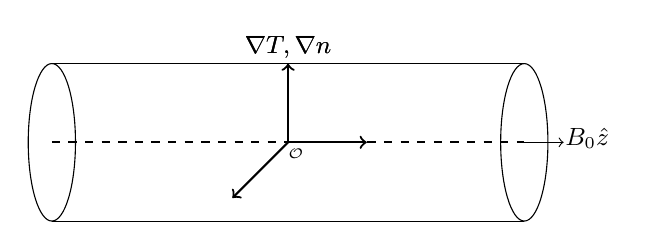
\begin{tikzpicture}[scale=1]
			% Cylinder axis from left to right
			(0,0) ellipse (0.3 and 1) % left cap
			(6,0) ellipse (0.3 and 1); % right cap (hidden)
			% Body
			(0,1) -- (6,1) arc (90:-90:1 and 0.3) -- (0,-1) arc (-90:90:1 and 0.3);
			% Front and back ellipses
			\draw (0,0) ellipse (0.3 and 1);
			\draw (6,0) ellipse (0.3 and 1);
			\foreach \angle in {0,90, 225}{
				\draw[->,thick] (3,0) -- ++(\angle:1);
			}\foreach \angle in {0,90}{
				\node at (3,1.2) {\small{$\nabla T, \nabla n$}} ++(\angle:1);
			}
			\node at (3.1,-0.15) {\tiny{$\mathcal{O}$}};
			% Cylinder outline
			\draw (0,1) -- (6,1);
			\draw (0,-1) -- (6,-1);
			\draw[dashed, thick] (0.0,0.0) -- (6.0,0.0);
			\draw[->] (6.0,0.0) -- (6.5,0.0);
			\node at (6.8,0.05) {\small{$B_0\hat{z}$}};
		\end{tikzpicture}
		\caption{Plasma Cil\'indrico con campo uniforme y transporte radial de part\'iculas y energ\'ia}
	\end{figure}

Se pueden ver que finalmente las relaciones de transporte radial, o flujo de part\'iculas y energ\'ia se pueden escribir como

  \begin{eqnarray}
    \Gamma_n &=& -A\left<\textbf{D}\cdot\nabla n\right>_{\partial V} \label{eq:partflux}\\
    \Gamma_E &=& -A\left<\pmb{\chi}\cdot\nabla T\right>_{\partial V} + \frac{3}{2}A\left<T\pmb{\Gamma}\right>_{\partial V}\label{eq:energyflux}
    \end{eqnarray}
    
  Las cantidades $\chi$ y $D$ deben ser estudiadas m\'as a fondo antes de asumir que son simplemente coeficientes, ya que podr\'an depender de la densidad $n$ y la temperatura $T$.

